\section{Sidebar: Probes settings}
    Now that you have create your outcome diagram, you can modify the probes settings to set the $dMax$ you want and the QTA you desire.

\subsection{Setting a QTA}
    You can set a QTA in the \textbf{"Set a QTA"} section, there you are presented with the possibility to:
    \begin{itemize}
        \item Select the probe for which you want to set the QTA.
        \item Set the QTA at the three percentiles (25\%, 50\%, 75\%), the text to the left indicates which percentile is which. You need to set the delay in seconds.
        \item The minimum amount of successful events you can allow, which is bigger than 75\%.
    \end{itemize}
    Of course, for the delay of the QTA at three percentiles, the delay at the percentile must be higher or equal than the delay at the previous percentile and higher than 0.
    
    By pressing \textit{"Save QTA settings"} you will save the QTA for the defined probe.

\subsection{Setting the parameters of a probe}
    You can set the parameters for a probe in its section.
    To the left you can select the probe you want to set the parameter for. 
    We provide a slider (which goes from -10 to 10) for the $n$ parameters, to the right of the slider, you can select the number of bins for the probe. The maximum delay calculated will be shown below.

    Once you press \textbf{"Save delay"}, a message to the erlang wrapper will be sent, which will set the maximum delay you have set in the wrapper.

    \begin{figure}[H]
        \begin{center}
            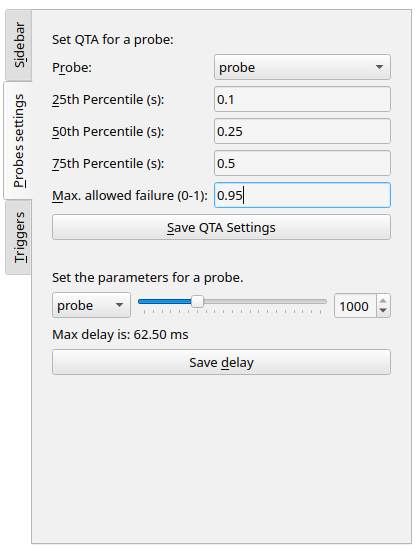
\includegraphics[width = \textwidth]{img/save_qta.png}
        \end{center}
        \caption{Probes settings tab. Above: QTA settings. Below: Probe parameters settings.}
    \end{figure}


